\documentclass[11pt,fleqn]{article}
\usepackage{../cs188,latexsym,epsf, amsmath,amsfonts,graphicx,url}
\lecture{8}
\def\title{Note \the\lecturenumber}
\begin{document}
\maketitle


\iffalse
\documentclass[11pt,fleqn]{article}
\usepackage{latexsym,epsf,amsmath,amsfonts,graphicx,url}

\title{Note 8}

\newcommand{\F}{\mathbb{F}}
\newcommand{\Z}{\mathbb{Z}}
\newcommand{\Q}{\mathbb{Q}}
\newcommand{\R}{\mathbb{R}}
\newcommand{\C}{\mathbb{C}}

\begin{document}

\maketitle
\fi


We have developed our techniques for probabilistic reasoning in the context of \textit{static} world, in which each random variable takes a single fixed value. For example, when probing the cavity, we assume that whatever tooth has a cavity remains cavitary during the process of probing; when forecasting the weather, we assume that whether the forecaster says a rainy day or not the weather does not change in that day. In many real-world problems, we want to reason about a sequence of observations. As a follow-up of the previous weather example, consider the task of monitoring every day's actual weather based on the historical weather forecasts. Unlike the previous example, here the \textit{dynamic} aspects of the problem are essential since the weather changes day by day. Other examples include robot localization where robot moves in a space and we want to know the robot's current location based on a sequence of range sensor observations, speech recognition where the task is to figure out the actual words people say based on a segment of rapidly changing acoustic signals, etc. 

\section{Markov Model}
Markov chain is a common model to capture the dynamics of the problem. 

\begin{center}	
	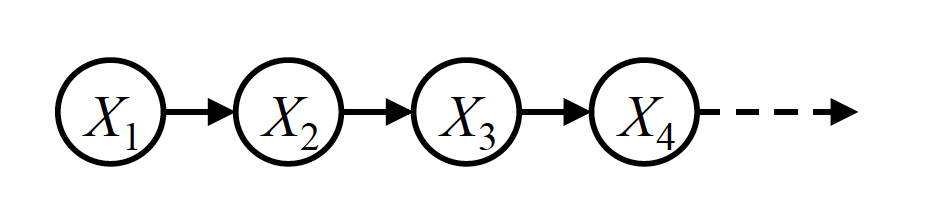
\includegraphics[width=10cm]{img/mc}
\end{center} 





\section{Hidden Markov Model}






\end{document}
